\chapter{Differential Geometry}
\label{chapter:differentialGeometry}

\section{Regular Surfaces and the First Fundamental Form}
%%%%%%%%%%%%%%%%%%%%%%%%%%%%%%%%%%%%%%%%%%
%%%
%%%     section regular surface
%%%
%%%%%%%%%%%%%%%%%%%%%%%%%%%%%%%%%%%%%%%%%%
Since all of the metrics in this thesis are based on the fact that 3D shapes can be modeled as regular surfaces the $\real^3$, this section will give some insight into the basics of the math behind them.
For all practical purposes these regular surfaces are approximated by piecewise linear triangular meshes, consisting of vertices and edges.
To begin with, we narrow down our choice of meshes to those, which are 2-dimensional manifolds without a boundary, so that we do not have to worry about boundary conditions.
The answer to the question, how a complex mesh can be represented mathematically, is given by the second chapter of \cite{do1976differential}:
The intuitive answer is to take pieces of a plane and to deform and arrange them, such that they cover the whole surface.
The only constraints to ensure the ability to apply differential geometry are, that the resulting surface is not allowed to have sharp points/edges or self-intersections.
A more rigorous definition is the following:
\begin{mydef}[regular surface]
	A subset $S \subset \real^3$ is a regular surface if, for each $p \in S$, there exists a neighborhood $V \in \real^3$ and a map $x:U \rightarrow V \cap S$ of an open set $U \subset \real^2$ onto $V \cap S \subset \real^3$ such that:
	\begin{enumerate}
		\item $x$ is differentiable. That means that if we write
			$$x(u,v) = (\mathbf{x}(u,v), \mathbf{y}(u,v), \mathbf{z}(u,v)), \quad (u,v) \in U,$$
			the functions $\mathbf{x}(u,v), \mathbf{y}(u,v), \mathbf{z}(u,v)$ have continuous partial derivatives of all orders in $U$.
		\item x is a homeomorphism. Since $x$ is continuous by condition 1, this condition requires that $x$ has an inverse $x^{-1}: V \cap S \rightarrow U$ which is continuous.
		\item For each $q \in U$, the differential $dx_q: \real^2 \rightarrow \real^3$ has full rank.
	\end{enumerate}
\end{mydef}
%%figure showing regular surface
\begin{figure}[h]
	\centering
	\includegraphics[width = 0.9\textwidth]{pictures/regular_surface}
	\caption{A graphical example of a regular surface: The points of the parameter domain $U$ are mapped to the surface $S$ by the parametrization $x$ with $p = x(q)$.
			The derivative of the map $dx_p$ maps tangent vectors of $U$ (in the basis $e_1,e_2$) to tangent vectors on $S$ (in the basis $dx_p(e_1), dx_p(e_2)$.}
	\label{fig:reg_surf}
\end{figure}
This definition states, that for every point on the surface there exists a neighborhood with a map $x$ which maps from the parameter domain $U \subset \real^2$ to $S$ (in correspondence to the plane patch from earlier) and the collection of all those neighborhoods defines the regular parametrized surface as can be seen in figure~\ref{fig:reg_surf}.
\begin{remark}
	The first condition ensures that we can use differential geometry on the regular surface, while the second one restricts the surface, such that it can not have intersections with itself.
	Even though the differential of the map $dx_p$ is covered later in this section, it can already be told that the third condition is responsible for the surface only having non-degenerated tangent planes.
\end{remark}

One of the important points of regular surfaces is, that its local properties do not change, if we use another parametrization.
Thankfully, it has already been proven, that there always exists a diffeomorphism that can transfer points from one parameter domain to the other and therefore make different maps interchangeable:
Let $p$ be a point on a regular surface $S$ and $x: U \rightarrow S$ and $y: V \rightarrow S$ be parametrizations of $S$ with $p \in x(U) \cap y(V) = W$.
Then the change of coordinates $h: y^{-1}(W) \rightarrow x^{-1}(W), h = x^{-1} \circ y$ is differentiable and has a differentiable inverse.
%\cite{do1976differential}[70ff]

Now that we have defined regular surfaces, the next step is to find a way to express functions defined on the surface.
Since we already know, that a regular surface is just a image of a two dimensional parameter domain, we can use that knowledge to define our function there.
\begin{mydef}[differentiable function on surfaces]
	Let $f$ be a function from an open subset $V \subset S$ of a surface $S$ to $\real$.
	Then $f$ is called differentiable at $p \in V$ if, for a parametrization $x: U \rightarrow S, p \in x(U) \subset V$, the composition $\tilde{f} = f \circ x$ is differentiable at $x^{-1}(p)$.
	$f$ is differentiable in V, if it is differentiable at all points of $V$.
\end{mydef}
%\cite{do1976differential}[72ff]
This means we can now transfer functions from one domain into the other, given a parametrization.

%%tangent planes
After defining how to transcribe functions between the parameter domain and the actual surface, we will now continue with the behavior of vectors under the differential map $x$.
Let us begin with the best visual concept of differentiating a map, the tangent plane.
The concept of a tangent plane is that at a certain point on the surface, the tangent vectors of all differentiable parametrized curves through that point constitute a plane.
\begin{mydef}[tangent plane]
	Let $x: U  \subset \real^2 \rightarrow S$ be a parametrization of a regular surface $S$ and let $q \in U$.
	The vector subspace of dimension 2, $dx_q(\real^2) \subset \real^3,$ coincides with the set of tangent vectors to $S$ at $x(q)$ and is called tangent plane to $S$ at $p = x(q)$ and will be denoted by $T_p(S)$.
\end{mydef}
Notice, that the above definition of the tangent plane is not dependent on the parametrization $x$.
The parametrization only determines the basis ${(\partial x/\partial u)(q), (\partial x/\partial v)(q)}$ of the tangent plane $T_p(S)$.
From here on out, they are abbreviated as $(\partial x/\partial u) = x_u$ and $(\partial x/\partial v) = x_v$.
Before we take a look at vectors specifically, we have to understand the concept of the differential of a map which was already used a few times in this thesis:
\begin{mydef}[differential of a map]
	Let $x: U \rightarrow S$ be a differential map and let $\alpha: (-\epsilon, \epsilon) \rightarrow U$ be a differential curve in the parameter domain with $\alpha(0) = q, \alpha'(0) = w$.
	The composition of them is called $\beta = x \circ \alpha$.
	Then the differential of $x$ at $q$ is
	$$dx_q(w) = \beta'(0).$$
\end{mydef}
Since $\beta$ is the image of $\alpha$ on the surface $S$, $dx_q$ maps tangent vectors from the parameter domain to tangent vectors of the surface by definition.
Also, $dx_q$ is not dependent on $\alpha$ but is solely a property of the differential map $x$ and it is a linear map.
This can be seen, if we apply the chain rule to the definition of $dx_q$ where $(u,v)$ are coordinates in $U$ and $(x,y,z)$ are coordinates in $\real^3$:
$$dx_q(w) = \beta'(0) = (x \circ \alpha)'(0) = x'(\alpha(0)) \cdot \alpha'(0) = \begin{pmatrix} \partial(x)/\partial(u) & \partial(x)/\partial(v) \\
																								\partial(y)/\partial(u) & \partial(y)/\partial(v) \\
																								\partial(z)/\partial(u) & \partial(z)/\partial(v)
																				\end{pmatrix}
	\begin{pmatrix} \partial u/\partial t \\ \partial v /\partial t \end{pmatrix} $$
Notice that the first matrix indeed does not depend on a specific $\alpha$.

%% first fundamental form
The last point in this section is the introduction of the first fundamental form, which is a replacement for the natural inner product on a surface $S$.
\begin{mydef}[first fundamental form]
	The quadratic form $I_p : T_q(s) \rightarrow \real$ on $T_q(S)$, defined by
	$$I_p(w) =  \langle w,w\rangle_p = |w|^2 > 0,$$
	is called the first fundamental form of the regular surface $S\subset\real^3$ at $p\in S$.
\end{mydef}
%\cite{do1976differential}[92] for two paragraphs
It can be used to determine geometric values like lengths of curves and areas of regions on regular surfaces without referring back to the ambient space.

Given a certain basis ${x_u, x_v}$ associated to a parametrization $x(u,v)$ at $p$, we can express the first fundamental form in that basis.
Since a tangent vector $w\in T_p(S)$ is the tangent vector to a parametrized curve $\alpha(t) = x(u(t),v(t)), t\in (-\epsilon,\epsilon)$, with $p = \alpha(0) = x(u_0,v_0)$, we obtain
\begin{align*}
	I_p(\alpha'(0)) &= \langle \alpha'(0),\alpha'(0)\rangle_p \\
					&= \langle x_u u' + x_v v',x_u u' + x_v v' \rangle_p \\
					&= \langle x_u ,x_u \rangle_p  (u')^2 + 2\langle x_u ,x_v \rangle_p u' v' + \langle x_v ,x_v \rangle_p (v')^2 \\
					&= E(u')^2 + 2Fu'v'+G(v')^2 \\
					&= \begin{pmatrix} u' & v' \end{pmatrix} \begin{pmatrix} E & F \\ F & G \end{pmatrix} \begin{pmatrix}u' \\ v'\end{pmatrix}
\end{align*}
where the values of the functions involved are computed for $t = 0$ and $E$,$F$ and $G$ are dependent on the basis ${x_u,x_v}$ of $T_p(S)$.
By letting p run in the coordinate neighborhood corresponding to $x(u,v)$ we obtain functions $E(u,v)$,$F(u,v)$ and $G(u,v)$ which are differentiable in that neighborhood.
These coefficients play important roles in many intrinsic properties of the surface.
Now we can even use two different vectors $(\alpha,\beta), (\delta,\gamma) \in T_p(S)$ to insert into the matrix notation to get the more general bilinear form of the first fundamental form:
$$I_p((\alpha, \beta),(\delta, \gamma)) = \begin{pmatrix} \alpha & \beta \end{pmatrix} \begin{pmatrix} E & F \\ F & G \end{pmatrix} \begin{pmatrix}\delta \\ \gamma\end{pmatrix}$$
One nice property of the first fundamental form is that it is invariant to isometries \cite{do1976differential}, which makes it a good candidate for a base of an intrinsic metric.

\section{Minimal Geodesics on Surfaces}
\label{section:geodesic}
%%%%%%%%%%%%%%%%%%%%%%%%%%%%%%%%%%%%%%%%%%
%%%
%%%     section geodesics
%%%
%%%%%%%%%%%%%%%%%%%%%%%%%%%%%%%%%%%%%%%%%%
One of the most fundamental metrics is the idea of constructing the shortest path between two points and define the length of that path as the distance between those two points.
In the Euclidean domain, this metric is defined by the Euclidean norm of the vector joining the two points.
On a regular surface, defining this distance is not as easy, since a lower dimensional set is embedded into a higher dimension.
The basic idea is, to find the shortest path along the surface from one point to the other and take its length as the distance.
It is commonly known, that such a path is a straight line and its generalization to curved surfaces is called a minimal geodesic, which will be defined during the course of this section.

Since a geodesic is definitely some kind of curve, we start by introducing the core concepts needed for the definition of a geodesic.
\begin{mydef}[parametrized curve]
	A parametrized curve $\alpha$ is the restriction of a differentiable mapping $( 0-\epsilon, l+\epsilon) \rightarrow S), \epsilon > 0$ to the interval $[0,l]$.
	The curve $\alpha$ is called to join two points $p,q \in S$ if and only if $\alpha(0) = p$ and $\alpha(l) = q$ and it is called regular, if its derivative $\alpha'(t)$ is nonzero for $t \in [0,l]$.
\end{mydef}
Now let $w(t)$ be a vector field along the curve $\alpha$.
Then $w$ is called differentiable, if for the parametrization $x(u,v)$ the vector field $w(t)$ can be written as $w(t) = a(t) \cdot x_u + b(t) \cdot x_v$, where $a$ and $b$ are differentiable functions.
Another important part is the covariant derivative of a vector field.
\begin{mydef}[covariant derivative]
	Let $\alpha(t)$ be a parametrized curve on $S$ with $\alpha(0) = p \in S, \alpha'(0) = y \in T_p(S)$ and a differential vector field $w(t)$ constricted to $\alpha$.
	The normal projection of the derivative of $w$ in respect to time $\frac{dw}{dt}(0)$ onto the tangent space $T_p(S)$ is called the covariant derivative at $p$ of the vector field $w$ relative to $y$:$\frac{Dw}{dt}(0)$
\end{mydef}
The covariant derivative is well-defined for differentiable vector fields and is furthermore intrinsic.
This can be seen, if we look at the expression for the covariant derivative:
$$\frac{Dw}{dt} = (a' + \Gamma^{1}_{1 1} a u' + \Gamma^{1}_{1 2} a v' + \Gamma^{1}_{1 2} b u' + \Gamma^{1}_{2 2} b v')x_u + (b' + \Gamma^{2}_{1 1} a u' + \Gamma^{2}_{1 2} a v' + \Gamma^{2}_{1 2} b u' + \Gamma^{2}_{2 2} b v')x_v$$
where $(u' v') = y$  and the $\Gamma$ are the so called Christoffel symbols, which are only dependent on first fundamental form and therefore $\frac{Dw}{dt}$ is an intrinsic property of the surface as shown in chapter 4.3 of \cite{do1976differential}.
A geometric interpretation of the covariant derivative would be the second derivative of the vector field $w$ as seen from the surface.
\begin{mydef}[parallel vectorfield]
	The vector field $w$ along the parametrized curve $\alpha$ is called parallel if it satisfies
	$$\frac{Dw}{dt} = 0 $$
	for all points on $\alpha$.
\end{mydef}
An example for parallel vector fields can be seen in figure~\ref{fig:parallel_vec}.
\begin{figure}[h]
	\centering
	\includegraphics[width = 0.9\textwidth]{pictures/parallel_vectorfield}
	\caption{Left: parallel vector field $w$ of a curve $\alpha$. Right: The second derivative of a curve $\alpha$ on the meridian of a sphere is normal to the surface of the sphere and therefore is a parallel vector field.}
	\label{fig:parallel_vec}
\end{figure}

%% picture
Now every aspect of the following definition has been introduced:
\begin{mydef}[geodesic curve]
	A non-constant, parametrized curve $\gamma: I \rightarrow S$ is called geodesic at $t \in I$ if the field of its tangent vectors $\gamma'(t)$ is parallel along $\gamma$ at $t$.
	Consequently, the curve $\gamma$ is called geodesic, if $\frac{D\gamma'}{dt} = 0 \forall t \in I$. \cite[238-246]{do1976differential}
\end{mydef}
To be a minimal geodesic, the curves length has to be less or equal to the length of any other piecewise regular curve on the surface.
\begin{example}
	If we look at the sphere $S^2$, its geodesic curves are obtained by intersecting the sphere with a plane passing through the center point of the sphere.
	This results in circle-shaped curves whose tangential vector field is parallel, since it is always pointing into the same direction if seen from the surface (see figure~\ref{fig:parallel_vec}).
	So there are at least two geodesics joining two points $p_1$ and $p_2$, just by following the intersection in different directions, starting from $p_1$.
	%TODO? vllt noch näher zu erklären, aber erstmal genug
	On the $S^2$ the minimal geodesic would be either the shorter arc joining $p_1$ and $p_2$ or, if they are antipodal points like the north and the south pole, there is an infinite number of minimal geodesics joining $p_1$ and $p_2$.
\end{example}
On the other hand, the existence of a minimal geodesic is not granted:
Let $p$ be a point on the minimal geodesic joining the points $p_1$ and $p_2$ (which are not a pair of antipodal points/sufficiently close) on the sphere $S^2$ and let the surface be $S^2-{p}$.
Then there exists no minimal geodesic between $p_1$ and $p_2$, since the only other geodesic joining them goes the long way around and is therefore longer than a piecewise regular curve almost equal to the minimal geodesic on $S^2$ except for going around the hole at $p$.
%TODO? picture?
One way to ensure the existence of a minimal geodesic is to constrain the surfaces to have certain properties.
%5.3 -P5 every compact surface is complete -> compact (closed and bounded [not inf]112 im text) also
%complete?
In general, most of the surfaces examined are both closed and bounded which means, they are compact.
As shown in \cite[331-332]{do1976differential}, compact surfaces are complete and we can use the theorem of Hopf and Rinow: \\
\begin{theorem}
	``Let S be a complete surface. Given two points $p,q$, there exists a minimal geodesic joining $p$ and $q$.'' \cite[333]{do1976differential} \\
\end{theorem}
Hence we can safely assume that there exists a minimal geodesic on the regular surfaces considered.
This approach is not very practical on actual meshes, since it needs a parametrization of the surface and comparing the length of all possible geodesic curves is not feasible.

\subsection*{Discretisation to triangulated meshes}
There are two main ways to compute shortest geodesic paths on triangulated meshes:
One is solving the Eikonal equation with the Fast Marching Method to approximate geodesics on the mesh as proposed by Kimmel and Sethian in \cite{kimmel1998computing}.
The second way, which will be used later in this paper, has been proposed by Mitchel, Mount and Papadimitriou (MMP) in 1987.
Their basic ideas are presented here, for further information, we refer to \cite{surazhsky2005fast}.
The fundamental idea is to use a simple parametrization of the geodesic distance on each edge and propagate the distance information starting from the source point over the whole surface.
Take note, that geodesics on a triangular mesh need to have two properties:
\begin{itemize}
	\item They need to be straight lines within each face.
	\item When crossing over an edge, the shortest paths need to correspond to a straight line if the faces are unfolded into a common plane.
\end{itemize}
Additionally, there are two kinds of vertices which need additional attention: boundary vertices and saddle vertices, which have a total angle greater than $2\pi$.
With this in mind, we can take a look at the MMP algorithm.
The main element of this are the so called windows, which bundle multiple shortest paths that traverse an edge into the same direction, into one tuple of six parameters.
%% need pictures of the different parameters + small picture for pseudo sources+distances

\paragraph{The window parameters}
\begin{figure}[h]
	\centering
	\includegraphics[width = 0.9\textwidth]{pictures/geodesics_parameters}
	\caption{Visualization of the window parameters}
	\label{fig:geo_param}
\end{figure}
Let's first assume, that the shortest path from the source vertex $v_s$ to the point $p$ does not pass through any boundary or saddle vertices.
In that case, all traversed triangles can be unfolded into a common plane, so that the path is a straight line in that plane.
If we now consider some neighboring points of $p$ whose shortest paths pass through the same sequence of faces, we get at set of straight lines emanating from $v_s$ intersecting the same edges.
So these paths are combined into one window and it is saved for the edge $e$ by first defining its width through determining the beginning and the end point of the window by $b_0, b_1 \in [0,||e||]$.
Additionally, the relative position of the source vertex to the window is encoded by the distance $d_0,d_1$ to the two window endpoints and a binary direction $\tau$.
In the case, that the path passes through one or more saddle/boundary vertices, let $s$ be the one closest to $p$.
All paths of $p$ and its neighboring points pass through $s$, which therefore is a (pseudo-)source for them.
The window now stores the distance information to $s$ as its source and an additional parameter that contains the distance of $s$ from $v_s$: $\sigma = D(s)$.
So the distance field $D$ over the window is described by the tuple $(b_0,b_1,d_0,d_1,\sigma,\tau)$ which are visualized in figure~\ref{fig:geo_param}.

\paragraph{Window propagation}
\begin{figure}[h]
	\centering
	\includegraphics[width = 0.9\textwidth]{pictures/geodesics_new_windows}
	\caption{Visualization of the three possible situations during the propagation step.}
	\label{fig:geo_new_windows}
\end{figure}
%% pictures of the propagation process (1,2,4 new windows)
To compute the distance function over the whole mesh, the windows are propagated over it.
Given a window $w$ on the edge $e_1$, the distance field will be propagated over a adjacent face $f$, resulting in new windows on the opposing edges $e_2,e_3$ of that face.
Since there are possibly already existing windows on those edges, we later need to intersect them with the existing ones and only keep the information of the shortest distances.
After again unfolding the mesh into a common plane, we extend the connections of the endpoints of $w$, $b_0$ and $b_1$, and the source $s$ until they intersect with one of the opposing edges.
This results in either one or two new windows, depending on whether or not there is an vertex in between the two intersection points.
Now we already have the values of $b_0', b_1'$ of the new window $w'$ and only need to compute the new distances between $s$ and the new endpoints to obtain $d_0'$ and $d_1'$.
The pseudosource distance $\sigma' = \sigma$ stays the same and the direction $\tau$ is assigned to point into the face $f$.

The special case of $w$ being adjacent to a saddle/boundary vertex $v$ results in a few additional windows.
Since shortest paths may pass through $v$, we need to add windows to the parts of the face, which can be reached through $v$ and are not already taken care of by the preceding steps.
As seen in figure~\ref{fig:geo_new_windows}, if $p_0$ is a saddle/boundary vertex and part of the window, the algorithm first generates the regular window on the edge $\overline{p_1p_2}$.
But additionally it adds windows to the darker blue part of the triangle, since those are the parts of the face, which can probably only be reached by passing through $p_0$.
These windows will have the pseudosource $p_0$ and $\sigma = D(p_0)$ is set accordingly.
This scenario is treated in a symmetric manner for the mirrored case where $p_1$ is part of the window.

\paragraph{Intersection of windows}
\begin{figure}[h]
	\centering
	\includegraphics[width = 0.9\textwidth]{pictures/geodesics_intersection}
	\caption{Left: initial situation before the intersection. Right: the starting and ending points of the two windows have been adjusted to the point $p$}
	\label{fig:geo_intersect}
\end{figure}
Once all new windows were created, we can intersect them with the existing ones, resulting in windows with the minimal distance.
Let $\delta$ be the non-empty intersection interval of two windows $w_1$ and $w_2$.
In the simple case, that one of the windows has a larger distance all over $\delta$, then $\delta$ is just cut away from its interval.
This leaves only intersections, were one window has a shorter distance on one end, while the other window is nearer to the source on the other end (figure~\ref{fig:geo_intersect}.
To intersect those two windows, we need to find the point $p \in \delta$  in between them, which is exactly as far away from the source in one window, as it is in the other.
This means, that $p$ has to fulfill the following condition:
$$||s_0 - p|| + \sigma_0 = ||s_1 - p|| + \sigma_1$$
This equation can be reduced to a quadric which has only one solution with the constraint $p \in \delta$.
Finally, we only need to adjust the boundaries $b_1$ of $w_1$ and $b_0$ of $w_2$ to match the point $p$ and recompute the endpoint distances.

\paragraph{Propagation order}
The described algorithm propagates the distance information from the source point outwards in a Dijkstra-like manner.
This means, that every time, a window is created or modified, it will be placed in a priority queue from which then the first window is taken and propagated across a face next.
Even though the algorithm computes the same result even without an specific ordering of the queue, the performance is increased, if the queue is ordered by the windows distance from the source.
Notice, that windows can be added, modified and removed in one step and the queue has to be updated accordingly.

During initialization, on each edge adjacent to the source vertex $v_s$ a window is created.
The distance fields on those windows are trivial, e.g. the distance every vertex adjacent to $v_s$ is equal to the edge length.
After that, one window is popped of the priority queue in each step and processed.

\paragraph{Construction of geodesic paths}
After the distance information was propagated throughout the whole mesh, it is easy to find the shortest/geodesic path from any given point $p$ to the source $s$.
In the most general case of $p$ lying on the interior of a face, we first collect all the windows on its edges and minimize the length of the path going from $p$ through the window to the source.
So in other words, we minimize $||p - p'|| + D(p')$ for all p' within those windows.

The next step is to trace back the path from $p'$ to $s$.
To do this, we take the direction $\tau$ of the window containing $p'$ and locate its pseudo-source $v_s$ using the distance information provided.
The next point in the backtracing process is obtained by intersecting the line $\overline{v_{s}p'}$ with the opposite edges of the face.
Now the algorithm is repeated with the window containing the intersection.

A special case again are pseudosources, which are boundary or saddle vertices:
To trace them back, we look at the adjacent windows and iteratively go through them, until we find one with a pseudosource different from the boundary/saddle vertex we are currently looking at.
Using that knowledge, we can compute the minimal geodesics and their lengths on triangulated surfaces like it can be seen in figure~\ref{fig:geo_paths}.
%picture of a mesh with geodesic curves on it
\begin{figure}[h]
	\centering
	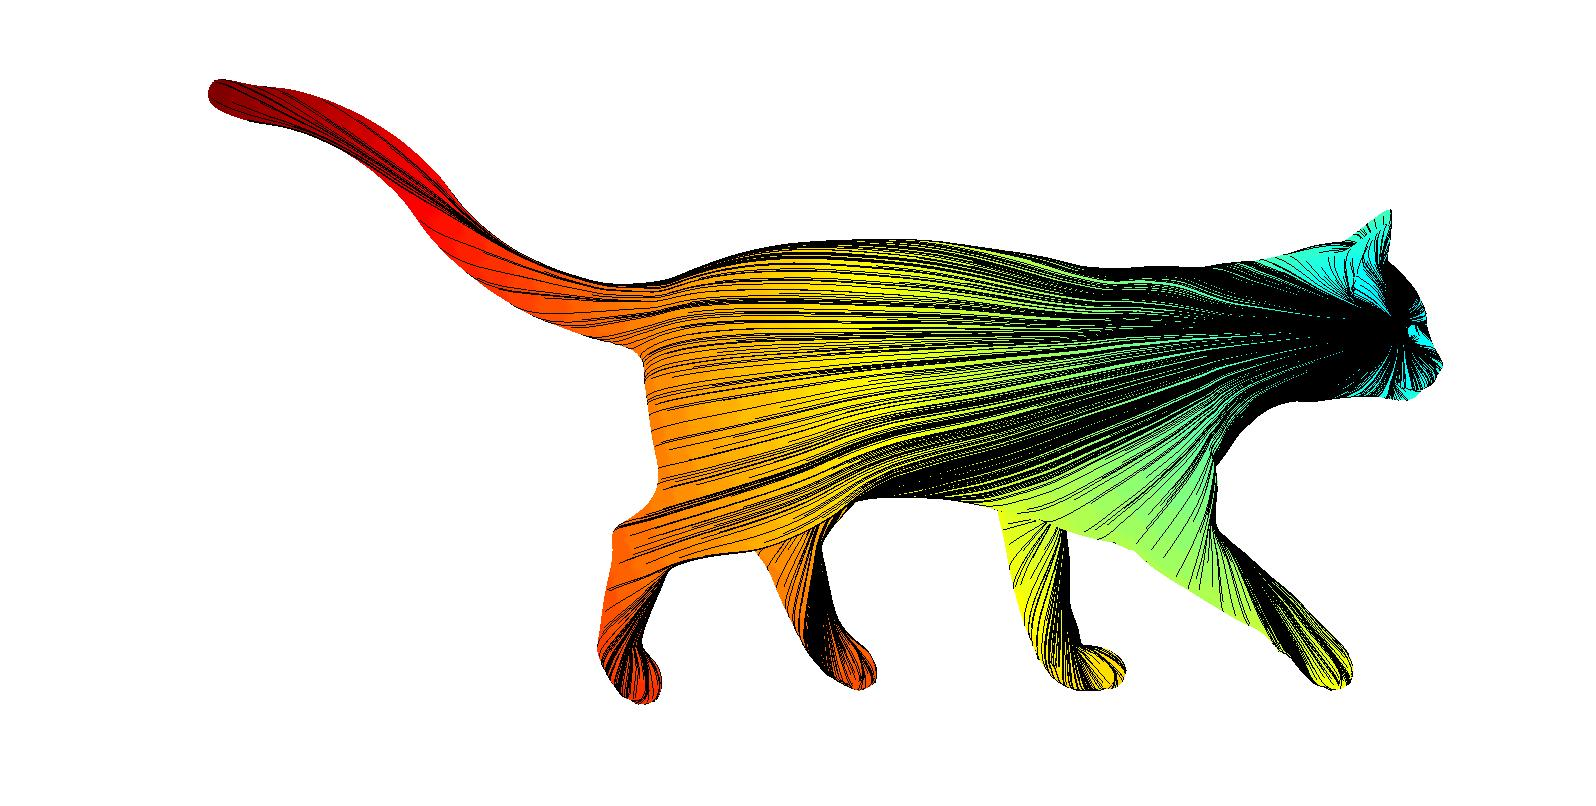
\includegraphics[width = 0.9\textwidth]{pictures/cat_geodesic_paths}
	\caption{A visualization of geodesic paths on the mesh of a cat. The plotted paths are the minimal geodesics connecting one point on the head to the other points.}
	\label{fig:geo_paths}
\end{figure}

\section{The Laplacian and Metrics based on its Eigenfunctions}
%%%%%%%%%%%%%%%%%%%%%%%%%%%%%%%%%%%%%%%%%%
%%%
%%%     section Laplacian
%%%
%%%%%%%%%%%%%%%%%%%%%%%%%%%%%%%%%%%%%%%%%%
%%laplacian is linear -> can be represented as a matrix
\subsection{The Laplacian on regular surfaces}
The Laplace-Beltrami operator (or Laplacian for short) on a regular surface is the restriction of the general Laplace operator onto the surface.
Geometrically, the Laplacian can therefore be seen as the second derivative of a function on a surface, in analogy to the one dimensional case of the Laplace operator in Euclidean space $\Delta f = f''$.
But the point we are interested in is that its eigenfunctions are orthogonal to each other and, even more interesting, the Laplace-Beltrami Operator only depends on the first fundamental form and therefore is invariant to isometries.

\subsubsection{Definition}
Since the Laplace operator is defined as the divergence of the gradient of a function $f$,
$$\Delta f = div(\nabla(f))$$
we first need to prove that those two functions are well defined on a regular surface.

\paragraph{The Gradient}
In Euclidean space $\mathbb{R}^n$, the gradient is defined as
$$\nabla f = \left(\frac{\partial f}{\partial x_{1}}, \dots, \frac{\partial f}{\partial x_{n}}\right).$$
The resulting vector points into the direction of the greatest increase of the function and its magnitude corresponds to the slope of the function.
By the Riesz Representation Theorem, it is also used to define the directional derivative $d f_{p}(v)$ of f at the point $p$ in the direction of the vector $v \in \mathbb{R}^n$:
\begin{equation}
	\langle \nabla f(p), v \rangle = d f_{p}(v)
	\label{eq:grad}
\end{equation}
Another way to define the directional derivative $d f_p(v)$ is to watch its behavior over time:
\begin{equation*}
	d f_p(v) = \frac{d}{dt_{|t=t_0}} f(p + tv)
\end{equation*}
or, in a more general way, by using $\gamma : (-\epsilon, \epsilon) \rightarrow \mathbb{R}^n \mbox{ fulfilling } \gamma(0) = p, \dot{\gamma}(0) = v$
\begin{equation*}
	d f_p(v) = \frac{d}{dt_{|t=t_0}} f(\gamma(t)).
\end{equation*}
Now the second equation can be used on a regular surface $S$, since it is not necessary to use $f(p+tv)$ which could possibly go out of $S$ but any $\gamma$.
If the directional derivative $df_p(v)$ of $f: S \rightarrow \mathbb{R}^n \mbox{ and } v \in T_p(S)$ is calculated, a $\gamma$ satisfying the conditions exists by the construction of $T_p(S)$, so that $df_p(v)$ exists and can be used to define the gradient on the manifold.
After converting \eqref{eq:grad} into the arithmetics of regular surfaces, it looks like this:
\begin{equation*}
	I_p(\nabla f(p),v) = d f_p(v) \mbox{ for } \forall v \in T_p(S)
\end{equation*}
This equation implies that exactly one $\nabla f$ exists for $v \in T_p(S)$ to satisfy the equation above.

\paragraph{The Divergence}
The divergence operator $div$ converts a vector field $V: S \rightarrow T_p(S)$ into a scalar field.
Even though the formula for doing so in the $\mathbb{R}^n$
\begin{equation}
	div\, V = \sum_{i=1}^{n} \frac{\partial V_i}{\partial x_i}
\end{equation}
seems complex, the idea behind it is simple:
It basically interprets the vector field as the definition of a flow, whose direction and volume in a certain point is defined by the corresponding vector.
The operator will then compute the current volume change under the influence of $V$.
It can be proven, that for a function $f$ with a compact support and a vector field V, the divergence is the negative adjoint operator to the gradient:\cite{polymesh}
\begin{equation}
	\langle V, \nabla f \rangle = \langle -div\, V, f \rangle
\end{equation}
Since we already know, that the first fundamental form of our surface is the equivalent of the inner product in Euclidean space and there exists a unique gradient for every $f$ on $S$, there also exists a unique function fulfilling the above equation.

\begin{mydef}[Laplace-Beltrami operator]
	Let $S$ be a regular Surface with $x:U\subset\real^2 \rightarrow S$ as its parametrization and $T_p(S)$ being its tangent plane.
	Then the Laplace-Beltrami operator is defined as
	$$\Delta f = div(\nabla(f))$$
\end{mydef}
Combining our knowledge about the gradient and the divergence together, we come to the conclusion that the Laplace-Beltrami-Operator is well-defined on regular surfaces.
It can even be expressed in the parameter domain of $S$, but again, since we are working on actual meshes, we will now take a look at the discretisation of our new defined operator on triangular meshes.

\subsubsection{Discretisation of the Laplacian and its eigenfunctions}
Since the Laplacian maps functions to functions, we first take a look at functions are represented on a mesh based on the approach in \cite{discretelaplacian2011}.
Generally a function $f$ is represented by its values at each vertex of the mesh.
The missing information about the function values inside the faces can be filled in by interpolation, for example by assuming that the function behaves linearly inside of every triangle.
To achieve this, we use the finite element method, which approximates a function $f$ by breaking it into a finite set of basis functions $\{\phi_i\}$.
The resulting representation of $f$ is a linear combination of the basis functions $\tilde{f} = \sum_i f_i \phi_i$ with weights $f_i \in \real$.
For triangulated meshes, the most natural choice of basis functions are the piecewise linear hat functions $\phi_i$ which equal one at their associated vertex and zero at all other vertices.

\paragraph{Computation of the Laplacian}
Next, we define the function $h = \Delta f$ and get the discretized representation $h = \sum_i h_i \phi_i$.
One could think that the Laplacian should vanish, since it is a second derivative and all hat functions $\phi_i$ are linear.
But due to Green's identity, by breaking up the integral into a sum over all triangles $\sigma$, it holds that
\begin{align}
	\langle \Delta f, \phi_j \rangle &= \sum_{k} \langle \Delta f, \phi_j \rangle_{\sigma_k} \\
	&= \sum_{k} \langle \nabla f, \nabla \phi_j \rangle_{sigma_k} + \sum_{k} \langle N \cdot \nabla f, \phi_j \rangle_{\partial \sigma_k}.
\end{align}
As long as the mesh has no boundary, the second sum vanishes since the normals $N$ of each edge of the mesh cancel each other out as adjacent triangles have mirrored normals.
Consequently, we are left with the term $\langle \nabla f, \nabla \phi_j \rangle$ for each triangle and as long as that term does not vanish, the resulting Laplacian is not zero.
Because $f$ is a linear combination, we can further simplify:
\begin{align}
	\langle \nabla f, \nabla \phi_j \rangle &= \sum_i f_i \underbrace{\langle \nabla \phi_i, \nabla \phi_j \rangle}_{C_{ij}} \\
	& = \frac{1}{2} \sum_{i \in neighbor(j)} (\cot \alpha_{ij} + \cot \beta_{ij})(f_i - f_j)\\
	& = (Cf)_j
	\label{eq:laplace:cotan}
\end{align}
where $f_i$ is the value of $f$ at the vertex $v_i$ and $\alpha_{ij},\beta_{ij}$ are the angles opposite of the edge between the vertices $v_i$ and $v_j$ on the adjacent faces.
Since we are searching for the coefficients $h_i$ of the Laplacian and $h$ is a linear combination, we can reformulate:
\begin{align}
	\langle h, \phi_j \rangle = \sum_i h_i \underbrace{\int \phi_i(x) \phi_j(x) dx}_{M_{ij}} = (Mh)_j
	\label{eq:laplace:mass}
\end{align}
%TODO berechnung von C und M ... vllt im appendix?
If we now combine \eqref{eq:laplace:cotan} and \eqref{eq:laplace:mass}, the result is a matrix representing the Laplace operator:
\begin{align}
	\langle h, \phi_j \rangle = \langle \Delta f, \phi_j \rangle
	Mh &= Cf \Rightarrow h = M^{-1}Cf = Lf
	\label{eq:laplace:final}
\end{align}
The matrix $L$ maps the coefficients of $f$ to the coefficients of $h = \Delta f$ and has the dimension of the number of vertices to the power of two.

\paragraph{Eigenfunctions of the Laplacian}
Because the Laplace-Beltrami operator is linear, it has to have eigenfunctions, which are used in the metrics later described.
Since we already showed that the Laplacian can be represented by a matrix $L$ to map functions to functions, the eigenvectors of $L$ represent functions on the mesh.
Using the Helmholtz equation and the knowledge obtained until now, we can use the matrices $M$ and $C$ to solve a generalized eigenvalue problem.
\begin{equation}
	\Delta f = \lambda f \Rightarrow M^{-1}C f = \lambda f \rightarrow Cf = \lambda M f
	\label{eq:laplacian:eigenvalue}
\end{equation}
As $C$ and $M$ are symmetric, we can use the QZ-algorithm as described in \cite{moler1973algorithm} to solve for the eigenvalues and eigenfunctions of the Laplacian.
Note that the QZ-algorithm returns a orthonormal (with respect to the $M$-inner product) basis of eigenvectors which in general is not unique, since eigenvectors can be scaled and still belong to the same eigenvalue.
Therefore the computed eigenfunctions can have switched signs due to the algorithm, but apart from that they are invariant to isometries as is the Laplacian.

\subsection{The Diffusion Distance}
The first metric to be discussed is the diffusion distance.
Specifically we consider heat diffusion over a surface, which is fully described by the heat kernel and associated with the Laplacian.
But instead of using the heat kernel itself, we use the so called Heat Kernel Signature (HKS) which was first proposed in \cite{sun2009concise}.
The heat kernel takes into account the heat transfer between all points at all time steps, whereas the HKS restricts the heat kernel to the temporal domain.
By preserving certain properties of the heat kernel, the HKS is a stable and isometry invariant metric on a mesh.

\paragraph{Heat Operator and Heat Kernel}
We start by introducing the basic facts about heat diffusion and the heat kernel needed to define the Heat Kernel Signature.
Let $S$ be a compact regular surface possibly with a boundary.
The heat diffusion process over $S$ is dominated by the heat equation
\begin{equation*}
	\Delta_S u(x,t) = -\frac{\partial u(x,t)}{\partial t}
	\label{eq:heat:eq}
\end{equation*}
where $\Delta_S$ is the Laplacian of $S$ and, if $S$ has a boundary, $u$ is required to satisfy the Dirichlet boundary condition $u(x,t) = 0 \: \forall x\in \partial S,t\in \real^+$.
The heat operator $H_t(f)$ describes the heat distribution after time $t$ given the initial heat distribution $f: S \rightarrow \real$, specifically fulfilling equation \eqref{eq:heat:eq} at all $T$ and converging to $f$ for $t \rightarrow 0$.
Both the heat operator and $\Delta_S$ are mapping real-valued functions defined on $S$ to another and it can easily be verified that they are related by $H_t = e^{-\lambda \Delta_S}$.
Hence both operators have the same eigenfunctions and if $\lambda$ is an eigenvalue of $\Delta_S$, then $e^{-\lambda t}$ is an eigenvalue of $H_t$ corresponding to the same eigenfunction.
\begin{mydef}[heat kernel]
	The heat kernel is the minimum function $k_t(x,y):\real^+ \times S \times S \rightarrow \real$ satisfying
	\begin{equation}
		H_tf(x) = \int_S k_t(x,y)f(y)dy.
		\label{eq:heat:kernel}
	\end{equation}
	For compact $S$ the heat kernel has the eigen-decomposition
	\begin{equation}
		k_t(x,y) = \sum_{i=0}^{\inf} e^{-\lambda_i t}\phi_i(x)\phi_i(y),
		\label{eq:heat:kernel:decomp}
	\end{equation}
	where $\lambda_i$ and $\phi_i$ are the $i^{th}$ eigenvalue and eigenfunction of the Laplace-Beltrami operator.
\end{mydef}
From a intuitive perspective, the heat kernel $k_t(x,y)$ is the amount of heat transferred from $x$ to $y$ in time $t$ from the starting heat distribution of one heat unit at $x$.
Another interpretation is that the heat kernel is the transition density function of Brownian motion on the regular surface.
This means that for $x,y\in S$, the heat kernel describes the probability of a random walker arriving at $y$ in time $t$ after starting at $x$.

%properties
According to \cite{sun2009concise} the most interesting properties of the heat kernel are that it is symmetric, isometry invariant, multiscale and stable.
Its symmetry is obvious, since it does not make a difference for the heat transfer from which point the heat originates, the amount of heat transferred stays the same.
That the heat kernel is isometry invariant is a consequence of the relation to the Laplacian which is invariant to isometries and only depends on intrinsic properties of the shape.
Due to this property, the heat kernel can be used to analyze shapes undergoing isometric deformations, for example matching articulated shapes.
The multiscale property comes from the heat kernels dependency on the time parameter.
It means that for small values of $t$, the function $k_t(x,\cdot)$ is mainly determined by small neighborhoods of $x$ and these neighborhoods grow bigger as $t$ increases.
This implies that $k_t(x,\dot)$ reflects the local properties of the shape around $x$ for small values of $t$, while it captures mainly the global structure of the shape from the point of view of $x$ for large values of $t$.
Lastly, the heat kernel being stable means that it is only slightly influenced by perturbations of the underlying regular surface.
The majority of deformable shapes in practice are not isometric and therefore a reliable metric should not be sensitive to small perturbations.
To explain the stability, we refer back to the heat kernels  interpretation as the transition probability of the Brownian motion on the surface.
Intuitively, this means that $k_t(x,y)$ is a weighted average of over all paths between $x$ to $y$ in time $t$, which should not be greatly affected by local perturbations.

\paragraph{Heat Kernel Signature}
We already showed that the  heat kernel is intrinsic, stable against noise and gives a multiscale characterization of the neighborhoods of a given point.
Now one could think about using the heat kernel itself as a point signature and assigning the family of functions $\{k_t(x,\cdot)\}_{t>0}$ as a signature of a point $x$.
Unfortunately, the complexity of this signature is extremely high, since one signature would be a function defined on $S \times \real^+$, the cross-product of the temporal and spatial domain.
The paper therefore proposes to restrict the heat kernel to the temporal domain as it contains a large amount of redundant information, mainly because the heat equation implies that the behavior of the spatial domain is heavily influenced by its changes over time.
\begin{mydef}[Heat Kernel Signature]
	Let $x$ be a point on the regular surface $S$, then its Heat Kernel Signature $HKS(x)$ is defined to be a function over the temporal domain:
	\begin{equation}
		HKS(x): \real^+ \rightarrow \real, HKS(x,t) = k_t(x,x) = \sum_{i = 0}^{\inf} e^{-\lambda_i t}(\phi_i(x))^2.
		\label{eq:hks:def}
	\end{equation}
\end{mydef}
The remaining question is, whether the Heat Kernel Signature $\{k_t(x,x)\}_{t>0}$ keeps all the information of $\{k_t(x,\cdot)\}_{t>0}$ or not.
One of the main results of \cite{sun2009concise} is the Informative Theorem which assures that the set of Heat Kernel Signatures is almost as informative as the more complex family of functions $\{k_t(x,\cdot)\}_{t>0}$.
\begin{theorem}[Informative Theorem]
	If the eigenvectors of the Laplace-Beltrami operators of two compact regular surfaces $M$ and $N$ are not repeated and $T$ is a homeomorphism from $M$ to $N$, then $T$ is isometric if and only if $k_t^M(x,x) = k_t^N(T(x),T(x))$ for any $x\in M$ and any $t>0$.
\end{theorem}
Additionally, the Heat Kernel Signatures at different points are defined over a common temporal domain, which makes them easy to compare.
Moreover, the HKS inherits many properties of the heat kernel, including being intrinsic, multi-scale and robust while still being inexpensive to store and easily commensurable.
Even though the Theorem states that the HKS is still informative, it requires the Laplace-Beltrami operator to not have repeating eigenvalues to hold in general.
One easy counterexample is  a sphere, where $k_t(x,x)$ is the same for all $x$, but it is clearly possible to construct non-isometric maps between two spheres of the same radius.  Although this example is degenerate, we will look whether or not this has an influence on shapes with intrinsic symmetries.

%TODO? Include scaled heat kernel signature?

\paragraph{Connection to Diffusion Distances}
The Heat Kernel Signature is closely related to diffusion maps and diffusion distances proposed by Lafon \cite{lafon2004diffusion} for data representation and dimensionality reduction.
The diffusion distance between $x,y \in S$ at time scale $t$ is defined as
\begin{equation}
	\begin{split}
		d_t^2(x,y) & = k_t(x,x) + k_t(y,y) - 2k_t(x,y) \\
		& = \sum_{i=0}^{\inf} e^{-\lambda_i t} (\phi_i(x) - \phi_i(y))^2.
	\end{split}
	\label{eq:hks:diffusion}
\end{equation}
This fact is pretty interesting, since we will see later on, that the Biharmonic distance as well as the Commute-time distance can be obtained by just replacing the heat kernel $k_t$ by their respective ``kernels''.
Notice, that the Heat Kernel Signature and its corresponding distance function is not scale invariant.
If we use the truncated sum from \eqref{eq:hks:diffusion}, we get a good approximation of the distance between two points.
Since the eigenvectors and eigenfunctions of the Laplace-Beltrami operator can be computed on a discretized mesh, we will use the truncated sum to approximate the distances between heat kernel signatures on a given mesh.
%TODO: scale invariant by setting t <- t/2\lambda_1 as in biharmonic

\subsection{Commute-time Distance}
The diffusion distance has got the problems, that for one it is not scale invariant and second that it depends on a time parameter, which has to be set for each shape specifically.
To solve the second problem, we can integrate the heat kernel over time, so that the result is no longer dependent on the time parameter:
\begin{equation}
	\begin{split}
		\int_0^{\inf} k_t(x,y)dt &= \int_0^{\inf} \sum_i e^{\lambda_i t}\phi(x)\phi(y) dt \\
		&= \sum_i \phi(x)\phi(y) \int_0^{\inf} e^{\lambda_i t} dt \\
		&= \sum_i \frac{1}{-\lambda_i} \phi_i(x) \phi(y) = g(x,y)
	\end{split}
	\label{eq:commute:kernel}
\end{equation}
The result is the commute-time kernel, which corresponds to the probability density function of a random walk of any length transitioning from point $x$ to $y$.
It can be used to define the commute-time distance in a similar fashion as the diffusion distance:
\begin{align}
	d_C^2(x,y) &= g_C(x,x) + g_C(y,y) -2g_C(x,y) \label{eq:commute:diffusion} \\
	&= \sum_{i=0}^{\inf} \frac{1}{-\lambda_i} (\phi(x)-\phi(y))^2. \label{eq:commute}
\end{align}
Furthermore, the commute-time distance is scale-invariant.
Note that the commute-time kernel is the harmonic Green's function of the Laplacian, which means that it fulfills the equation $\Delta \int g_C(x,y) f(y) dy  = f(x)$ for a given $f$.
The disadvantage of this is that the harmonic Green's function has a singularity at the diagonal, which means that \eqref{eq:commute:diffusion} is not defined in the continuous case.

\subsection{The Biharmonic Distance}
The biharmonic distance was proposed by Lipman, Rustamov and Funkhouser after reviewing the above described metrics on shapes in their paper \cite{lipman2010biharmonic}.
Their new distance operator is quite similar to the diffusion distance and the commute-time distance, but they exchanged the diffusion kernel with the Green's function of the biharmonic differential equation.
In the continuous case, the biharmonic distance can be defined using the eigenvectors and eigenvalues of the Laplace-Beltrami operator
\begin{equation}
	d_B(x,y)^2 = \sum_{i=0}^{\inf} \frac{(\phi_i(x) - \phi_i(y))^2}{\lambda_i^2}.
	\label{eq:biharmonic}
\end{equation}
This definition is only slightly different from the other two distances, the only part changing is the factor in font of the difference between the two eigenvectors.
While the biharmonic distance has a factor of $1/\lambda_i^2$, the power of the $\lambda$ in the definition of the commute-time distance is one and the factor of the diffusion distance is $e^{-\lambda_it}.$
So even though it is a seemingly minor change, the behaviour and the properties of the distance functions differ largely.
The basic idea behind this is that it is related to how fast the normalized $\lambda_i$ in the factors decay:
if the decay is to slow it will produce a logarithmic singularity at the diagonal of the harmonic Green's function (like $\sum_i 1/\lambda_i ~ \sum_i 1/i$).
On the other hand, if the decay is to fast, the eigenvectors with high frequencies are basically ignored and the distance becomes ``too global''.
The paper states, that the factor of $1/\lambda_i^2$ provides a good balance as it decays fast enough to be shape-aware over the whole mesh and slow enough to get good local properties around the source point.

The biharmonic distance as defined in \eqref{eq:biharmonic} can further be written to fit the diffusion distance formulation with a different kernel:
\begin{equation}
	\begin{split}
		d_B^2(x,y) & = \sum_{i=0}^{\inf} \frac{|\phi_i(x)|^2}{\lambda_i^2} + \sum_{i=0}^{\inf} \frac{|\phi_i(x)|^2}{\lambda_i^2} - 2 \sum_{i=0}^{\inf} \frac{\phi_i(x) \phi_i(y)}{\lambda_i^2}\\
		& = g_B(x,x) + g_B(y,y) - 2g_B(x,y).
	\end{split}
	\label{eq:biharmonic:diffusion}
\end{equation}
using the Green's function $g_B(x,y)$ of the biharmonic operator $\Delta^2$, which means that it satisfies the relation
\begin{equation}
	\Delta_{(x)}^2 \int g_B(x,y)f(y)dy = f(x)
	\label{eq:greensfunction}
\end{equation}
for smooth enough $f$.
This information can used to discretize the biharmonic distance by obtaining the discretized $g_B$ from \eqref{eq:greensfunction} and applying it to \eqref{eq:biharmonic:diffusion} to obtain the biharmonic distance on the mesh.
Another way to practically compute it is to approximate the distance by using the truncated sum, as it is the standard methodology for approximating the diffusion distance.
We compute the first $N$ eigenfunctions of the discrete Laplacian and computing $d_B(x,y)$ as follows:
\begin{equation}
	\tilde{d}_B(x,y)^2 = \sum_{i=0}^N \frac{(\phi_i(x) - \phi_i(y))^2}{\lambda_i^2}.
	\label{eq:biharmonic:practical}
\end{equation}
Although the error bound is (in general) linear in $1/K$ this approximation provides considerable speedup in trade-off of accuracy over the exact computation.
Additionally, since the approximate distance uses a fixed set of eigenvectors it is smooth.

